%-------------------------------------------------------------------------
\chapter{\babTiga}
%--------------------------------------------------------------------------
This chapter details the research methodology employed in this study. It includes descriptions of the dataset used, the overall system architecture, modifications made to the YOLO11 model, and the performance evaluation metrics applied to assess the effectiveness of the proposed approach.

\section{Dataset}
This research utilizes two primary datasets for training and evaluating the object detection models: the Dataset for Object Detection in Aerial Images (DOTA) and the Small Object Detection dAtaset (SODA). Both datasets are specifically designed for aerial imagery and present unique challenges for object detection tasks.

\subsection{DOTA Dataset}
The DOTA (Dataset for Object deTection in Aerial images) is a large-scale geospatial dataset widely used as a baseline for oriented object detection \cite{xia2019dotalargescaledatasetobject}. It is built from 2,806 high-resolution aerial images collected from different sensors and platforms, including Google Earth, to ensure a wide diversity of acquisition conditions. The images span from approximately $800 \times 800$ to $4,000 \times 4,000$ pixels, and together provide 188,282 annotated instances belonging to 15 common object categories such as plane, ship, storage tank, stadiums, harbor, bridge, large and small vehicles, helicopter, roundabout, and swimming pool. DOTA is split into training, validation, and test subsets with proportions of $1/2$, $1/6$, and $1/3$ respectively, which facilitates standard benchmarking protocols. Each instance is annotated with an Oriented Bounding Box (OBB) defined by four vertices $(x_i, y_i)$ arranged clockwise, which makes the dataset particularly suitable for aerial scenarios where objects appear at arbitrary rotations. The combination of extreme scale variation, dense object populations, and varying aspect ratios makes DOTA a challenging benchmark for evaluating object detection algorithms in aerial imagery. Figure \ref{fig:instances-dota} illustrates several instances from the DOTA dataset.

\begin{figure}
    \centering
    \includegraphics[width=1.0\textwidth]{pictures/Dataset - DOTA.jpg}
    \caption{Instances from the DOTA dataset.}\label{fig:instances-dota}
\end{figure}

\subsection{SODA Dataset}
The second dataset used in this research is the Small Object Detection dAtaset (SODA) benchmark \cite{Cheng_2023}, which contains two subsets tailored for driving (SODA-D) and aerial (SODA-A) scenarios. SODA-D spans 24,828 high-resolution street-level images with 278,433 instances labeled with Horizontal Bounding Boxes, while SODA-A focuses on aerial imagery and is the subset used in this research.

SODA-A comprises 2,513 aerial images harvested from Google Earth, each at an average resolution of $4761 \times 2777$ pixels to preserve the fine structure of tiny targets. The dataset contains 872,069 objects distributed over 9 classes, including Airplane, Helicopter, Small-vehicle, Large-vehicle, Ship, Container, Storage-tank, Swimming-pool, and Windmill. Data splits follow a 40\% / 25\% / 35\% ratio for training, validation, and testing, respectively. Similar to DOTA, annotations use Oriented Bounding Boxes (OBB) to capture rotated objects, but SODA-A explicitly targets the small-object challenge: objects with area under 1024 pixels are considered small, and the average instance size is only 14.75 pixels, with many instances qualifying as "Extremely Small" (area < 144 pixels). The dataset also exhibits extreme density, with some images containing over 11,000 instances, which compounds occlusion and background interference issues. These characteristics make SODA-A a demanding benchmark for evaluating detection performance on small, densely packed aerial targets. Figure~\ref{fig:instances-soda} shows several instances from SODA-A.

\begin{figure}
    \centering
    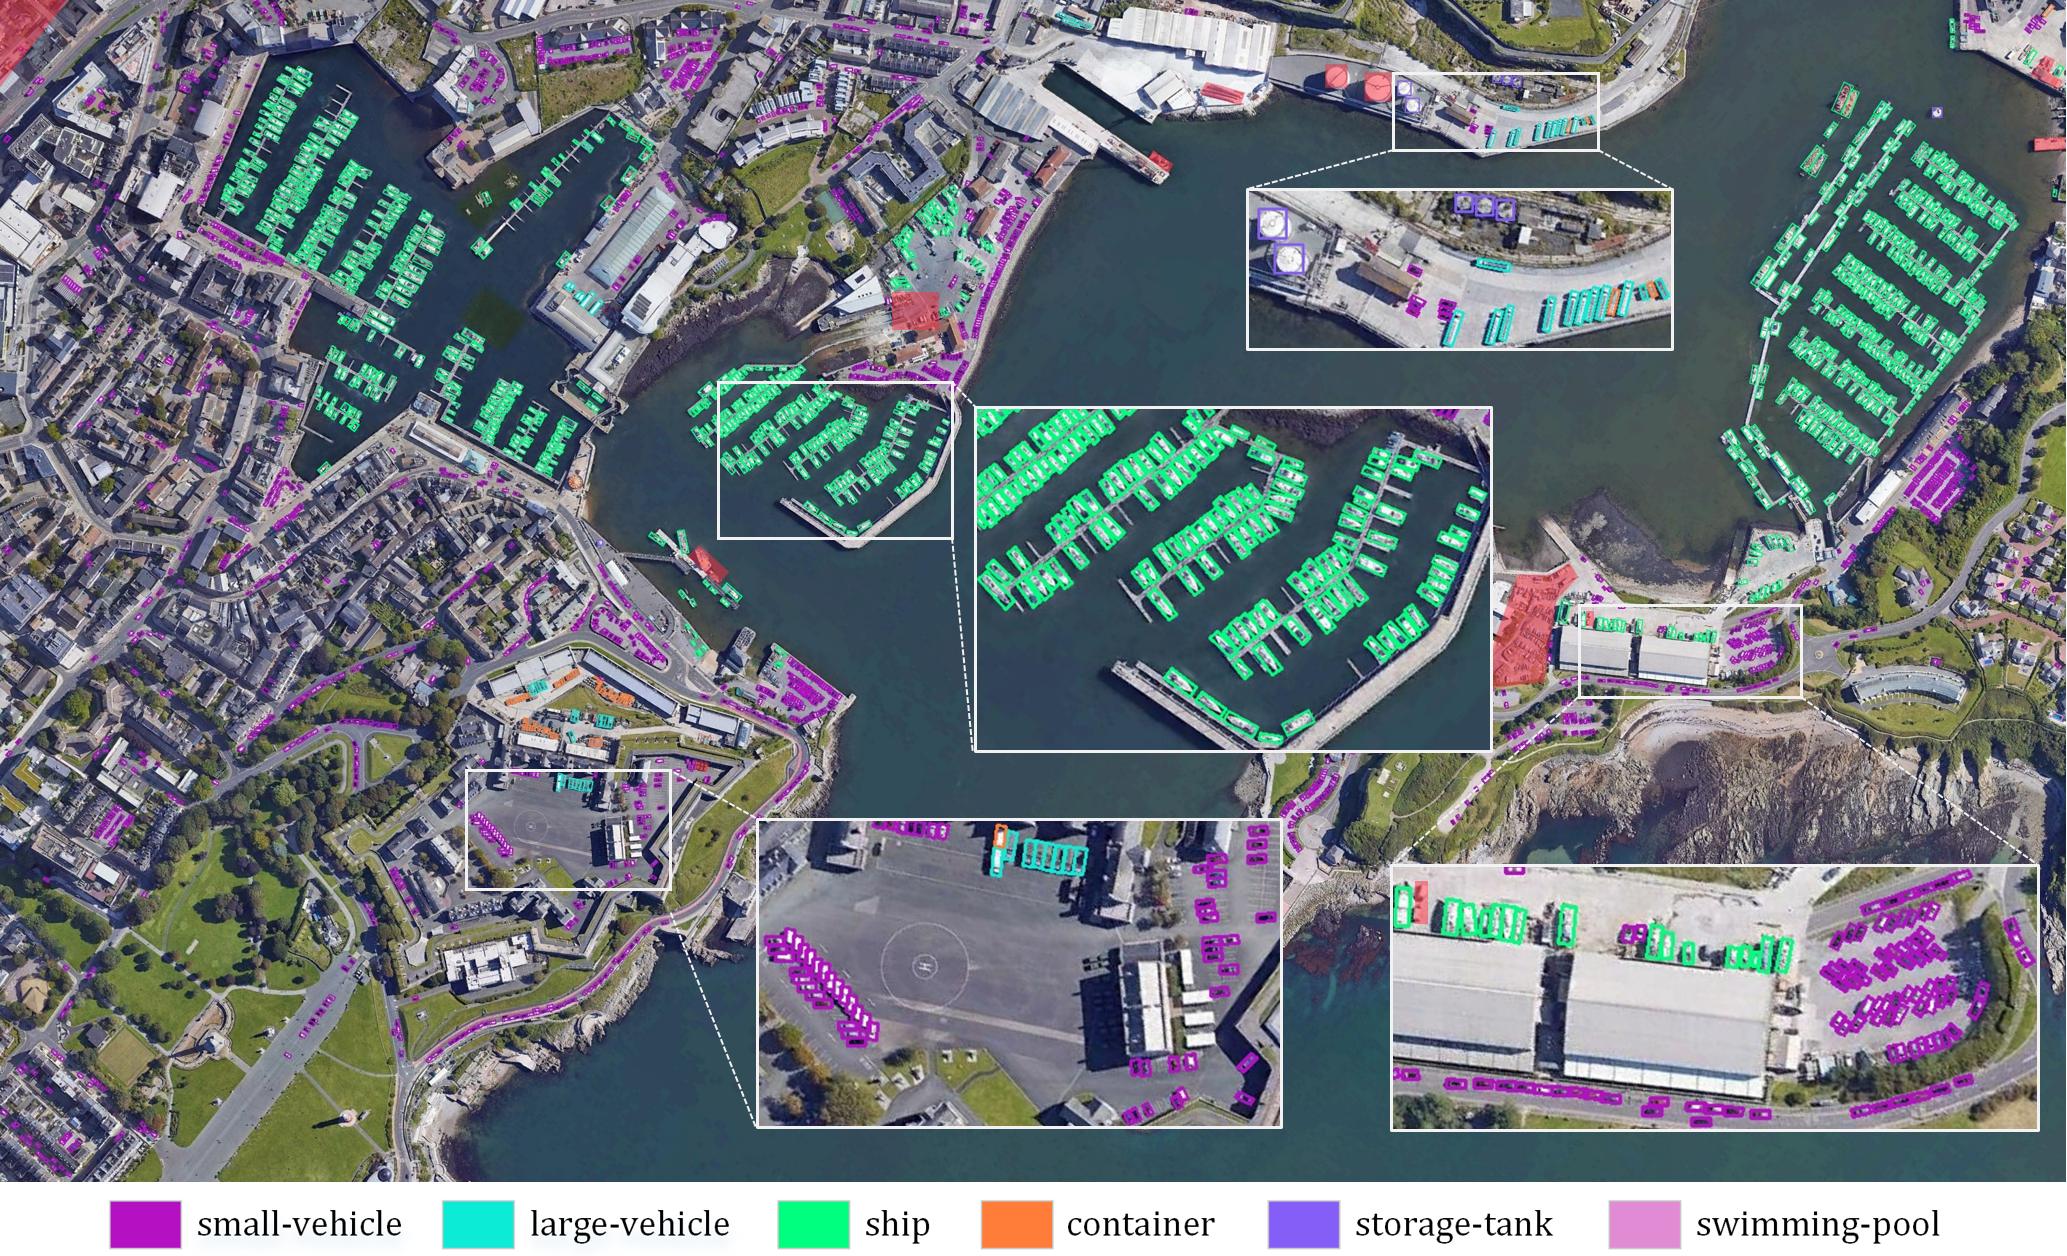
\includegraphics[width=1.0\textwidth]{pictures/Dataset - SODA-A.png}
    \caption{Instances from the SODA-A dataset.}
    \label{fig:instances-soda}
\end{figure}

The following Table~\ref{tab:dataset-summary} summarizes the key features of both datasets used in this research.

\begin{table}[htbp]
    \centering
    \caption{Summary of DOTA and SODA-A Datasets.}
    \label{tab:dataset-summary}
    \resizebox{\textwidth}{!}{
    \begin{tabular}{|l|l|l|}
        \hline
        \multicolumn{1}{|c|}{\textbf{Feature}} & \multicolumn{1}{c|}{\textbf{DOTA}} & \multicolumn{1}{c|}{\textbf{SODA-A}} \\
        \hline
        Domain & General Aerial Detection & Small Object / Dense Aerial Detection \\
        Images & 2,806 & 2,513 \\
        Instances & 188,282 & 872,069 \\
        Categories & 15 & 9 \\
        Annotation Type & Oriented Bounding Box (OBB) & Oriented Bounding Box (OBB) \\
        Key Challenge & Scale Variation, Orientation & Extremely Small Objects, High Density \\
        \hline
    \end{tabular}
    }
\end{table}

\section{System Process Architecture}
Figure~\ref{fig:system-process-architecture} illustrates the overall Experiment and Testing flow used in this research. The process begins with dataset preparation, where images and annotations from DOTA and SODA-A are standardized and converted into the annotation format required by the Ultralytics YOLO framework. The prepared dataset is then partitioned into training, validation, and testing subsets according to each dataset's predefined allocation ratios.

\begin{figure}
    \centering
    \includegraphics[width=0.6\textwidth]{pictures/Proposal Thesis - Experiment Diagram.png}
    \caption{System Process Architecture.}
    \label{fig:system-process-architecture}
\end{figure}

Next, the modified YOLO11 model is trained on the training set while monitoring validation performance to guide early stopping or further architecture tuning. When a trained checkpoint surpasses the established baseline, it is saved for later testing; otherwise, additional architectural modifications or hyperparameter adjustments are applied and the training loop repeats. The saved model is eventually loaded during the testing phase, where inference is performed on the unseen test set and the predicted boxes are compared to the ground-truth annotations to compute the evaluation metrics in this research. This system-wide process ensures that data collection, model development, and evaluation are tightly coordinated, which is essential for improving accuracy and efficiency in detecting aerial objects.

% ===================================================================

\section{Modified YOLO11 Architecture}

The baseline YOLO11 is highly optimized for general object detection but exhibits specific limitations when applied to aerial imagery, particularly regarding oriented and small objects. These limitations stem from the fixed geometric structures in standard convolutional layers, which struggle to capture the arbitrary orientations and scale variations typical in aerial views. Furthermore, the local receptive fields of standard CNNs restrict the modeling of long-range dependencies, making it difficult to identify small objects within complex backgrounds. To address these challenges, this research proposes YOLO11-DCN-DA, a hybrid architecture that integrates Deformable Convolutional Networks (DCN) and Deformable Attention mechanisms. Specifically, C3k2\_DCN modules replace standard C3k2 units in the backbone and neck to enhance geometric adaptability, while Deformable Attention blocks are added for context-aware feature fusion. As shown in Figure~\ref{fig:modified-yolo11-architecture}, these modifications are strategically placed where feature extraction is most critical rather than being applied uniformly across the network.

\begin{figure}
    \centering
    \includegraphics[width=1.0\textwidth]{pictures/Proposal Thesis - Proposed Architecture.png}
    \caption{Comparison of the (a) Baseline YOLO11 Architecture and (b) Proposed YOLO11-DCN-DA Architecture.}
    \label{fig:modified-yolo11-architecture}
\end{figure}

\subsection{Integration of C3k2\_DCN Module}
The fundamental building block of the YOLO11 backbone is the C3k2 module, an evolution of the Cross Stage Partial (CSP) bottleneck designed to optimize gradient flow. In its standard form, the internal bottleneck relies on $3 \times 3$ convolutions with a fixed sampling grid. This rigidity prevents the network from effectively aligning its receptive field with rotated objects, such as ships or vehicles in aerial views.

To address this, we introduce the C3k2\_DCN module. This custom block modifies the internal bottleneck structure by replacing the standard spatial convolution with a Modulated Deformable Convolution (DCNv2) layer. The modification process involves three key steps:

\begin{enumerate}
    \item{Split and Branching}\\
    Consistent with the CSP design principle, the input tensor is first processed by a $1 \times 1$ convolution and then split into two branches. This preserves the gradient flow benefits of the original architecture.
    \item{Offset Regression Branch}\\
    In the processing branch, a parallel lightweight convolutional layer is introduced. This layer takes the input feature map and predicts a dense offset field. For a kernel size of $3 \times 3$, this layer outputs a tensor with $27$ channels at each spatial location: $18$ channels for the $x$ and $y$ coordinate offsets ($\Delta p$) and $9$ channels for the modulation scalars ($\Delta m$).
    \item{Adaptive Sampling}\\
    The DCNv2 layer utilizes these learned offsets to deform the sampling grid. This effectively ``stretching'' or ``rotates'' the kernel's receptive field to align with the geometric structure of the target object, capturing semantic features that would otherwise be missed by a fixed grid.
\end{enumerate}

Figure~\ref{fig:c3k2_block_comparison} details the internal structure of the proposed C3k2\_DCN module. The module were strategically deployed in the medium and large stages of the Backbone and Neck, where high-level semantic information is richest and geometric transformation modeling is most critical.

\begin{figure}
    \centering
    \includegraphics[width=0.8\textwidth]{pictures/Proposal Thesis - C3k2 Block Comparison.png}
    \caption{Comparison between (a) Standard C3k2 module and (b) Proposed C3k2\_DCN module with deformable convolutions on bottleneck.}
    \label{fig:c3k2_block_comparison}
\end{figure}

\subsection{Deformable Attention Block Implementation}

While DCN enhances local geometric adaptability, detecting small objects in dense clusters requires a mechanism to capture global context and suppress background noise. Standard global attention mechanisms (like in Vision Transformers) compute relationships between all pixel pairs, resulting in quadratic computational complexity ($O(H^2 W^2)$), which is prohibitive for high-resolution feature maps.

To solve this, we implement a custom DeformableAtten block that wraps the Multi-Scale Deformable Attention (MSDeformAttn) mechanism into a CNN-compatible module. This block is designed to operate on 4D tensors ($B, C, H, W$) typically found in YOLO architectures, acting as a bridge between the CNN backbone and the feature fusion neck.

The implementation of this block involves a specific sequence of operations to translate between the spatial domain of CNNs and the sequence domain of attention mechanisms:

\begin{enumerate}
    \item{CNN-to-Sequence Transformation}\\
    The core MSDeformAttn operator expects input in a sequence format. Our wrapper first flattens the spatial dimensions of the input feature map ($H \times W$) into a sequence of query elements of length $N = H \times W$. This transformation prepares the data for the attention mechanism while preserving the feature dimensionality $C$.

    \item{Reference Point Generation}\\
    Unlike standard attention which is location-agnostic, Deformable Attention requires a set of reference points for each query element. Our implementation generates a normalized 2D grid $p_q \in [0, 1] \times [0, 1]$ corresponding to the spatial locations of each pixel in the feature map. These reference points serve as the ``anchor'' locations from which the attention mechanism learns to sample.
    \begin{equation}
        p_{q(i,j)} = \left( \frac{j + 0.5}{W}, \frac{i + 0.5}{H} \right)
    \end{equation}
    where $(i, j)$ are the spatial coordinates. This grid is generated dynamically based on the input feature map size, ensuring the block can handle varying resolutions.

    \item{Sparse Deformable Attention}\\
    The flattened features and generated reference points are passed to the MSDeformAttn module. For each query element, the module predicts a small set of sampling offsets relative to its reference point. It then samples features from these offset locations using bilinear interpolation and aggregates them. This sparse sampling reduces the complexity to linear time $O(HW)$, allowing the model to capture long-range dependencies without processing every pixel pair.

    \item{Feed-Forward Network (FFN) and Residuals}\\
    Following the standard Transformer design, the output of the attention mechanism is processed through a Feed-Forward Network (FFN). Our implementation includes normalization layers (LayerNorm) and residual connections around both the attention module and the FFN to facilitate gradient flow and training stability.
    \begin{equation}
        x = x + \text{Dropout}(\text{MSDeformAttn}(x, p_q))
    \end{equation}
    \begin{equation}
        x = \text{LayerNorm}(x)
    \end{equation}

    \item{Sequence-to-CNN Reconstruction}\\
    Finally, the processed sequence is reshaped back into the original 4D tensor format ($B, C, H, W$). This allows the feature map to be seamlessly passed to subsequent convolutional layers in the Neck.
\end{enumerate}

Figure~\ref{fig:deform_attn_block} illustrates the data flow within the Deformable Attention block. This block is placed at the end of the Backbone after the SPPF module, to refine the highest-level features with global context before multi-scale fusion occurs.

\begin{figure}
    \centering
    \includegraphics[width=1.0\textwidth]{pictures/Proposal Thesis - DefformableAttn Block.png}
    \caption{Deformable Attention implementation block.}
    \label{fig:deform_attn_block}
\end{figure}

% ====================================================================

\section{Performance Evaluation Metrics} 
In this research, the performance of the modified YOLO11 model is evaluated using standard object detection metrics, primarily focusing on Mean Average Precision (mAP) at different Intersection over Union (IoU) thresholds. Others metrics such as Precision, Recall, and F1-Score are also computed to provide a comprehensive assessment of the model's detection capabilities, especially in handling oriented and small objects in aerial imagery. To quantify computational cost, we also track the number of model parameters (Params) and Floating Point Operations(FLOPs), ensuring that accuracy improvements remain practical for real-world deployment.

\subsection{Precision}
Precision measures the proportion of correctly predicted positive instances (true positives) out of all instances predicted as positive (true positives + false positives). It reflects the model's ability to avoid false alarms.

\begin{equation}
    \mathrm{Precision} = \frac{TP}{TP + FP}
\end{equation}

where \( TP \) is the number of true positives and \( FP \) is the number of false positives.

\subsection{Recall}
Recall measures the proportion of correctly predicted positive instances (true positives) out of all actual positive instances (true positives + false negatives). It indicates the model's ability to detect all relevant objects.

\begin{equation}
    \mathrm{Recall} = \frac{TP}{TP + FN}
\end{equation}

where \( TP \) is the number of true positives and \( FN \) is the number of false negatives.

\subsection{F1-Score}
The F1-Score is the harmonic mean of Precision and Recall, providing a single metric that balances both aspects of model performance. It is particularly useful when the class distribution is imbalanced.

\begin{equation}
    \mathrm{F1\text{-}Score} = 2 \times \frac{\mathrm{Precision} \times \mathrm{Recall}}{\mathrm{Precision} + \mathrm{Recall}}
\end{equation}

\subsection{Mean Average Precision (mAP)}
Mean Average Precision (mAP) is the primary metric used to evaluate the object detection performance of the model. It is calculated by averaging the Average Precision (AP) across all object classes. AP is derived from the Precision-Recall curve for each class, which plots precision against recall at various confidence thresholds. The mAP is computed at different IoU thresholds (e.g., mAP@0.5, mAP@0.50-95) to assess how well the model detects objects with varying degrees of overlap with ground truth boxes. 

\begin{equation}
    \mathrm{mAP} = \frac{1}{N} \sum_{i=1}^{N} AP_i
    \label{eq:map}
\end{equation}

where \( N \) is the number of classes and \( AP_i \) is the Average Precision for class \( i \).

\subsection{Number of Parameters (Params)}
The number of parameters (Params) in the model quantifies its complexity and size. It is calculated by summing all learnable weights and biases across all layers of the neural network. A lower number of parameters generally indicates a more efficient model, which is beneficial for deployment in resource-constrained environments.

\begin{equation}
    \mathrm{Params} = \sum_{i=1}^{L} (W_i + B_i)
\end{equation}

where \( L \) is the number of layers, \( W_i \) is the number of weights in layer \( i \), and \( B_i \) is the number of biases in layer \( i \).

\subsection{Floating Point Operations (FLOPs)}
FLOPs measures the computational efficiency of the model by counting the number of floating-point operations required to process a single input image. It provides insight into the model's speed and resource requirements, which are critical for real-time applications.

\begin{equation}
    \mathrm{FLOPs} = \sum_{i=1}^{L} F_i
\end{equation}

where \( L \) is the number of layers and \( F_i \) is the number of floating-point operations in layer \( i \).